\documentclass[tikz,border=4pt]{standalone}
\usepackage{amsmath,amssymb}
\usetikzlibrary{positioning,fit,backgrounds,arrows.meta,shapes.geometric}

\begin{document}
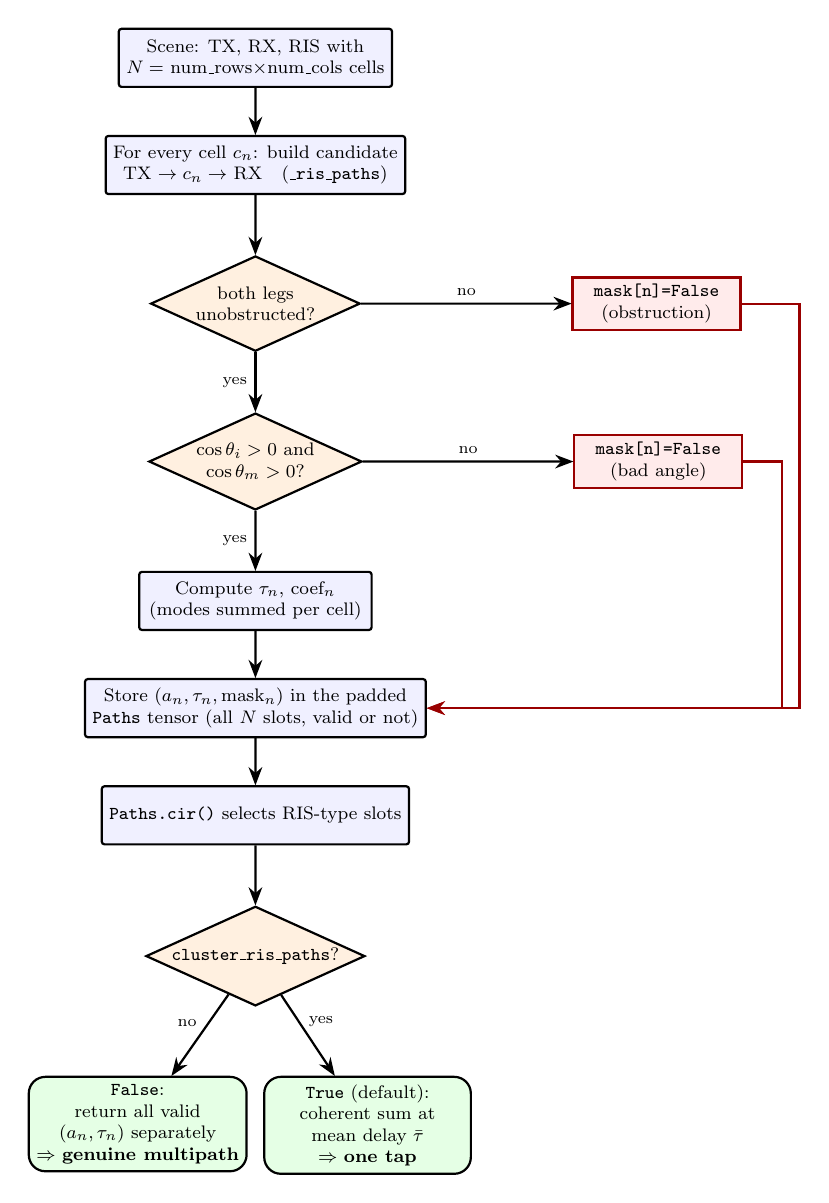
\begin{tikzpicture}[
  >=Stealth, thick, node distance=6mm and 12mm,
  scale=0.82, every node/.append style={scale=0.82},
  proc/.style={rectangle, draw=black, rounded corners=1pt, fill=blue!6,
               align=center, minimum width=3.6cm, minimum height=0.9cm,
               font=\footnotesize},
  dec/.style={diamond, draw=black, fill=orange!12, align=center,
              aspect=2.2, inner sep=1pt, font=\footnotesize},
  term/.style={rectangle, rounded corners=6pt, draw=black, fill=green!10,
               align=center, minimum width=3.2cm, minimum height=0.8cm,
               font=\footnotesize},
  bad/.style={rectangle, draw=red!60!black, fill=red!8, align=center,
              minimum width=2.6cm, font=\footnotesize, inner sep=3pt}
]

\node[proc] (scene) {Scene: TX, RX, RIS with\\ $N=$ num\_rows$\times$num\_cols cells};
\node[proc, below=of scene] (cand) {For every cell $c_n$: build candidate\\ TX $\to c_n \to$ RX \ \ (\texttt{\_ris\_paths})};
\node[dec, below=of cand, yshift=-2mm] (obst) {both legs\\ unobstructed?};
\node[bad, right=of obst, xshift=18mm] (obstfail) {\texttt{mask[n]=False}\\ (obstruction)};
\node[dec, below=of obst, yshift=-2mm] (ang) {$\cos\theta_i>0$ and\\ $\cos\theta_m>0$?};
\node[bad, right=of ang, xshift=18mm] (angfail) {\texttt{mask[n]=False}\\ (bad angle)};
\node[proc, below=of ang, yshift=-2mm] (coef) {Compute $\tau_n$, coef$_n$\\ (modes summed per cell)};
\node[proc, below=of coef] (store) {Store $(a_n,\tau_n,\text{mask}_n)$ in the padded\\ \texttt{Paths} tensor (all $N$ slots, valid or not)};
\node[proc, below=of store] (cir) {\texttt{Paths.cir()} selects RIS-type slots};
\node[dec, below=of cir, yshift=-2mm] (cluster) {\texttt{cluster\_\allowbreak ris\_paths}?};
\node[term, below left=12mm and -6mm of cluster] (false) {\texttt{False}:\\ return all valid\\ $(a_n,\tau_n)$ separately\\ $\Rightarrow$ \textbf{genuine multipath}};
\node[term, below right=12mm and -6mm of cluster] (true) {\texttt{True} (default):\\ coherent sum at\\ mean delay $\bar\tau$\\ $\Rightarrow$ \textbf{one tap}};

\draw[->] (scene) -- (cand);
\draw[->] (cand) -- (obst);
\draw[->] (obst) -- node[above,font=\scriptsize]{no} (obstfail);
\draw[->] (obst) -- node[left,font=\scriptsize]{yes} (ang);
\draw[->] (ang) -- node[above,font=\scriptsize]{no} (angfail);
\draw[->] (ang) -- node[left,font=\scriptsize]{yes} (coef);
\draw[->] (coef) -- (store);
\draw[->] (store) -- (cir);
\draw[->] (cir) -- (cluster);
\draw[->] (cluster) -- node[above,font=\scriptsize,xshift=-2mm]{no} (false);
\draw[->] (cluster) -- node[above,font=\scriptsize,xshift=2mm]{yes} (true);
\draw[->, red!60!black] (obstfail.east) -- ++(9mm,0) |- (store.east);
\draw[->, red!60!black] (angfail.east) -- ++(6mm,0) |- (store.east);

\end{tikzpicture}
\end{document}
